%%%%%%%%%%%%%%%%%%%%%%%%%%%%%%%%%%%%%%%%%
% University/School Laboratory Report
% LaTeX Template
% Version 3.1 (25/3/14)
%
% This template has been downloaded from:
% http://www.LaTeXTemplates.com
%
% Original author:
% Linux and Unix Users Group at Virginia Tech Wiki 
% (https://vtluug.org/wiki/Example_LaTeX_chem_lab_report)
%
% License:
% CC BY-NC-SA 3.0 (http://creativecommons.org/licenses/by-nc-sa/3.0/)
%
%%%%%%%%%%%%%%%%%%%%%%%%%%%%%%%%%%%%%%%%%

%----------------------------------------------------------------------------------------
%	PACKAGES AND DOCUMENT CONFIGURATIONS
%----------------------------------------------------------------------------------------

\documentclass{article}

\usepackage[version=3]{mhchem} % Package for chemical equation typesetting
\usepackage{siunitx} % Provides the \SI{}{} and \si{} command for typesetting SI units
\usepackage{graphicx} % Required for the inclusion of images
\usepackage{natbib} % Required to change bibliography style to APA
\usepackage{amsmath} % Required for some math elements 
\usepackage{gensymb}

\setlength\parindent{0pt} % Removes all indentation from paragraphs

\renewcommand{\labelenumi}{\alph{enumi}.} % Make numbering in the enumerate environment by letter rather than number (e.g. section 6)

%\usepackage{times} % Uncomment to use the Times New Roman font


%Code packages

\usepackage[utf8]{inputenc}
\usepackage{listings}
\usepackage{color}
% Code packages end


%----------------------------------------------------------------------------------------
%	DOCUMENT INFORMATION
%----------------------------------------------------------------------------------------

\title{Duffing Oscillator Sections\\ Class Twelve Summary\\ PHY 230} % Title

\author{Avi \textsc{Vajpeyi}} % Author name

\date{\today} % Date for the report

\begin{document}

\maketitle % Insert the title, author and date



% If you wish to include an abstract, uncomment the lines below
% \begin{abstract}
% Abstract text
% \end{abstract}

%----------------------------------------------------------------------------------------
%	SECTION 1
%----------------------------------------------------------------------------------------

\section{Objective - C and the Wave application}

For the past two weeks we have been working on objective c applications. We began by making a basic one in which we learned how to change the window name, and alter the color of the background. We then created a 'converter' app, in which we learned how to get text inputs and output data onto a window.We used this knowledge to convert miles to kilometers, and learned about various 'attributes' of text fields.\\

We moved on to working with more complex problems after that. We made an application where we were able to generate and display a polygon of user defined sides. In this application, we also let the user chose the colors of the shape, and the background. The user can also rotate the polygon and we eventually added an animation feature which rotated the polygon automatically. Figure\ref{poly} is a picture of the polygon application.\\


\begin{figure}[h]
	\caption{Screenshot of the Polygon app}
	\centering
	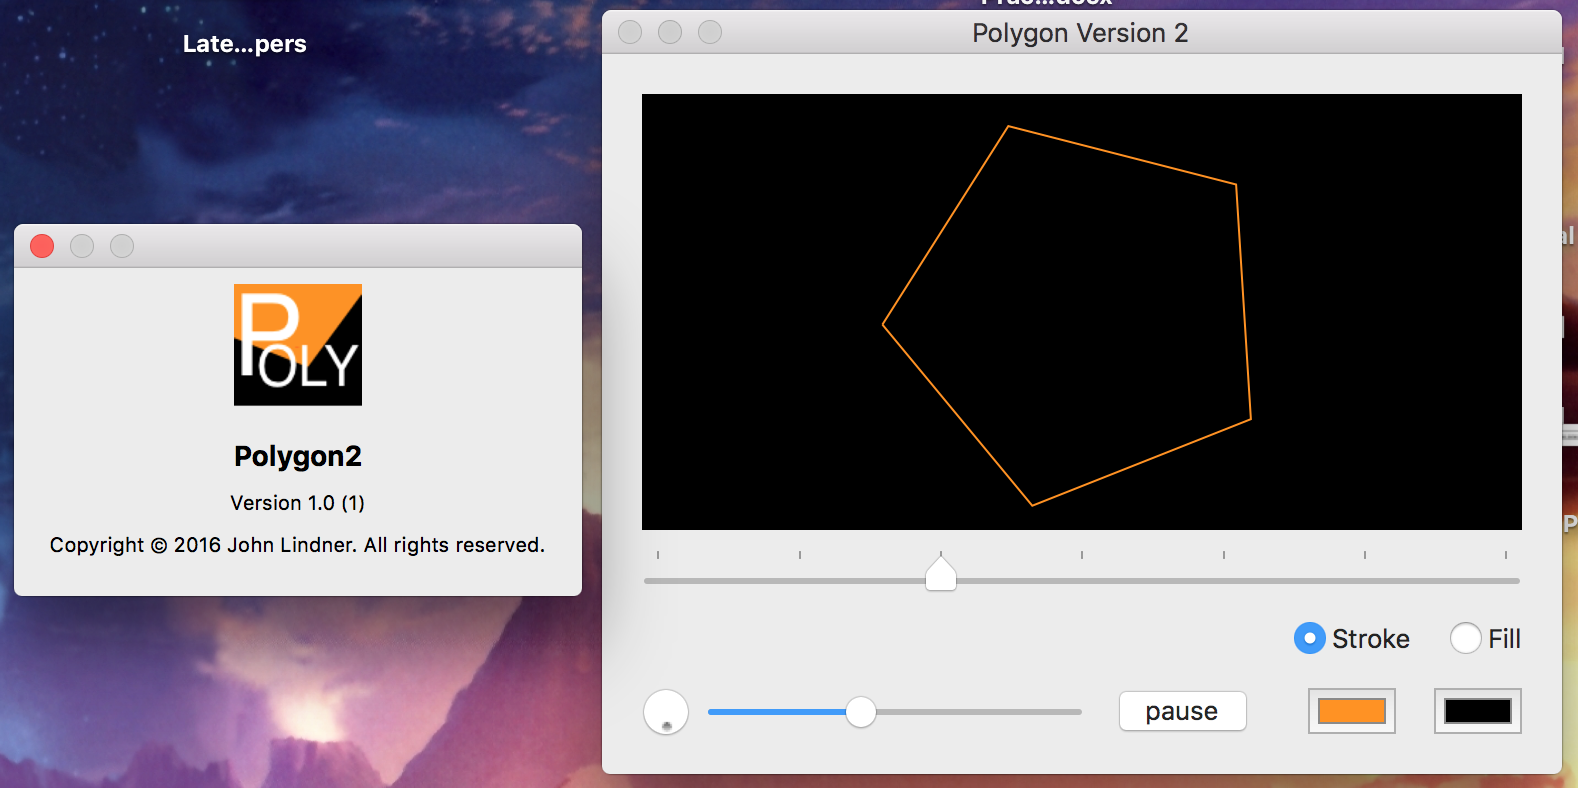
\includegraphics[width=0.5\textwidth]{poly} \label{poly}
\end{figure}

 
 
 We then moved onto begin work with the 'wave on a string' application. We were first given some theory on waves, and how we can model a wave on a string mathematically using a Gaussian. This was slightly confusing, however, it began to make sense as we discussed how the formulae could be implemented in Objective-C for our simulation.  
 
 While creating the simulation, I spent a long time making the wave appear. Towards the end of the class on Monday, I discovered that my program was correct, it was just that there was a integer division error that I had overlooked. I found this very amusing, as this was the very mistake we had discussed in length the first week of class.
 
 On Wednesday, we worked on animating the wave, and introducing options for boundary conditions, initial conditions and preferences such as colors of the wave and background. The figure \ref{poly} is a screenshot of the final version of the app. 
 
 
 
 \begin{figure}[h]
 	\caption{Screenshot of the Wave on a String app}
 	\centering
 	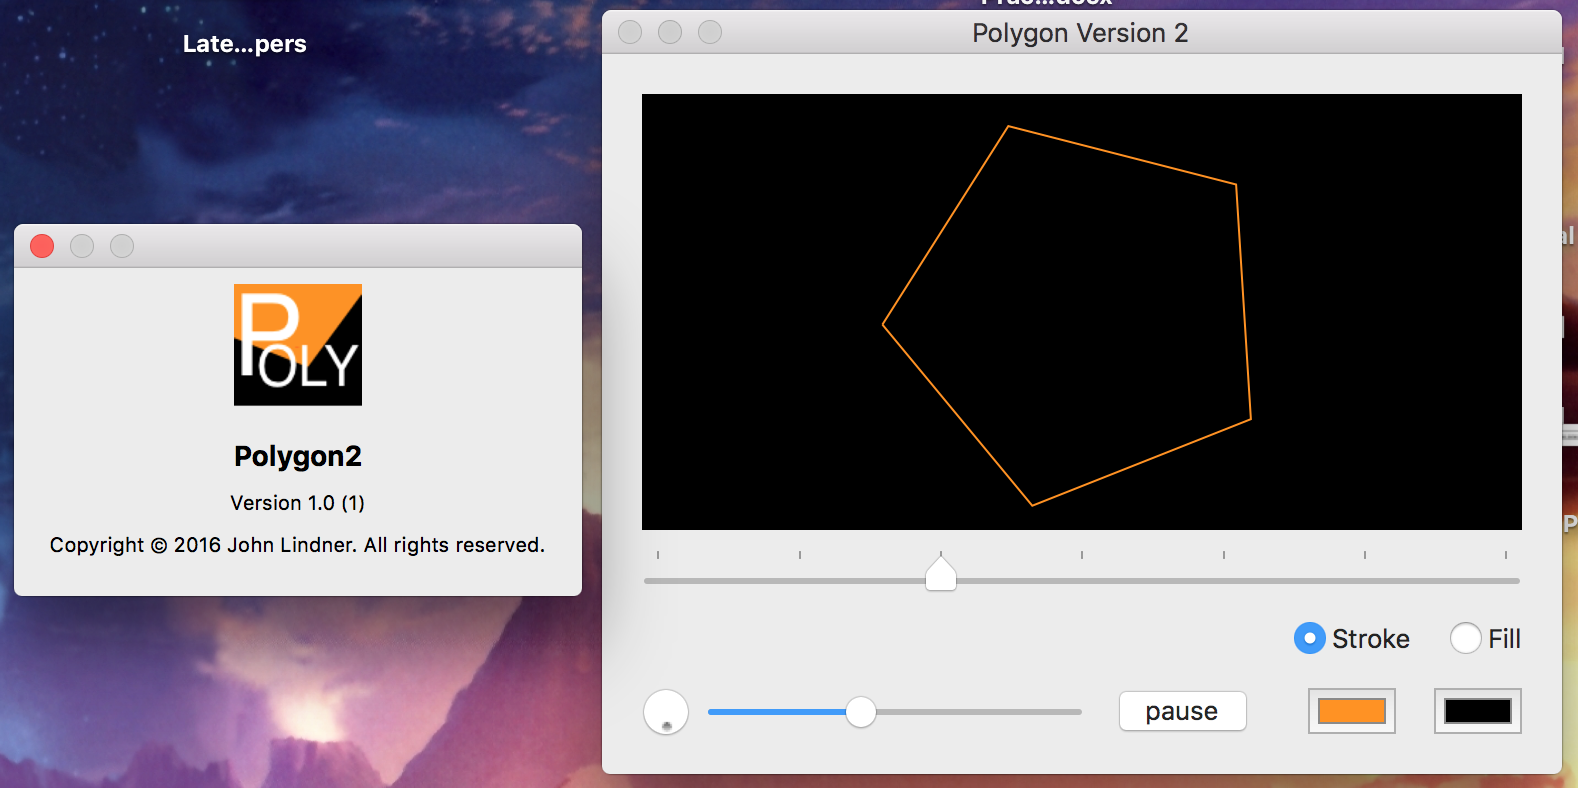
\includegraphics[width=0.5\textwidth]{poly} \label{wave}
 \end{figure}
 
 As seen from the figure, the user can pause or reset the animation. The user can also chose from four different boundary conditions. The fixed condition acts as though the string has been tied to a solid at both ends of the window. The Free 
 
 The most challenging aspect of this part of the project was dealing with the wrap around, or the 'periodic' boundary condition.\\  
 Use Xcode and its Interface Builder, along with Obj-C++ and the Cocoa APIs, to create a simulation of waves on a string. Enable the user to pause or reset the animation, toggle the initial conditions between a stationary pulse and a solitary moving pulse, toggle the boundary conditions among fixed or free or infinite or periodic, change the string colors and the background using color wells, change the string width using a slider, change the drawing style from stroke to fill. Add an application icon and archive a executable app.
 
 
%----------------------------------------------------------------------------------------


\end{document}